\item  The Web Module:

The module provides a portal based, web responsive front end that allows a user to get access to the application facets.


\textbf{Sections}
\begin {itemize}


\item {Login/out}\\
The buzz system does allow user name u0000000n (with n being any single number starting from 1) and password "password" to login and out of the buzz system.

\begin{figure}[h!]
  \centering
    \reflectbox{%
      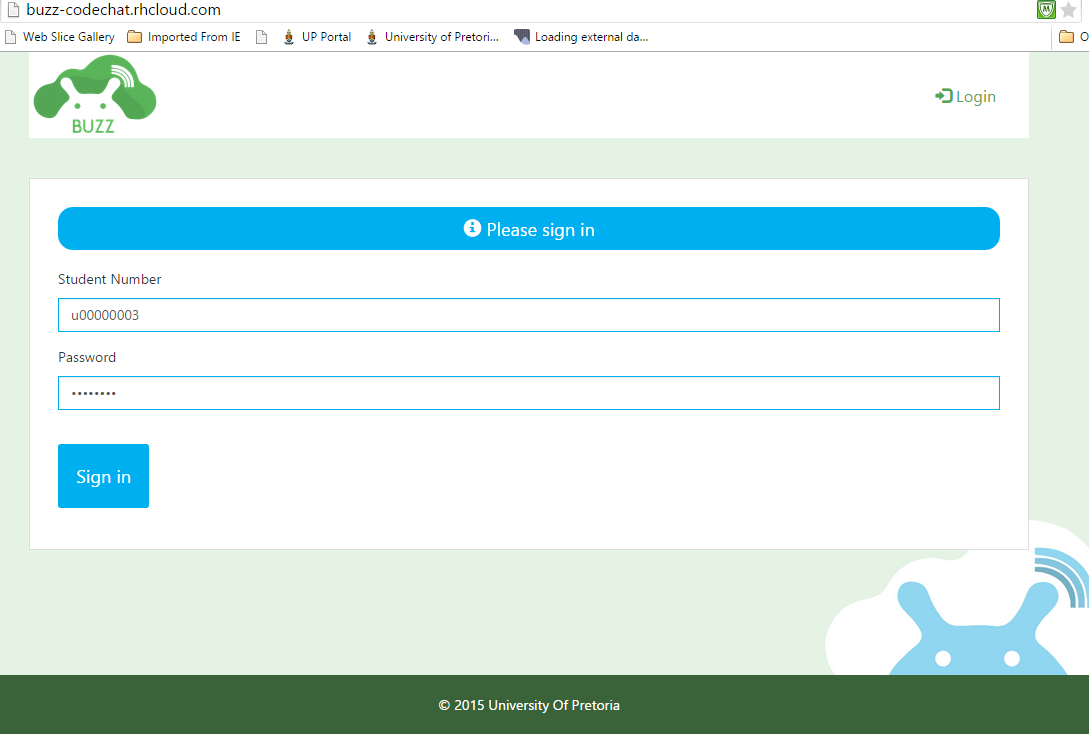
\includegraphics[width=0.5\textwidth,height=4cm]{loginadministrative(whatBdid)}}
  \caption{login format }
\end{figure}


\item personalization and configuration\\
A user cannot configure a dashboard type of view or buzz space, no functionality or options of such where provided.
\\

\item 	Accessibility of functionality\\
Access to a service does not depend on a user's role on a buzz space or a users status on that space, There is no form of grouping, all users are the same and have the same privileges and authorisations, basically all users have access to everything in the system.



\begin{figure}[h!]
  \centering
    \reflectbox{%
      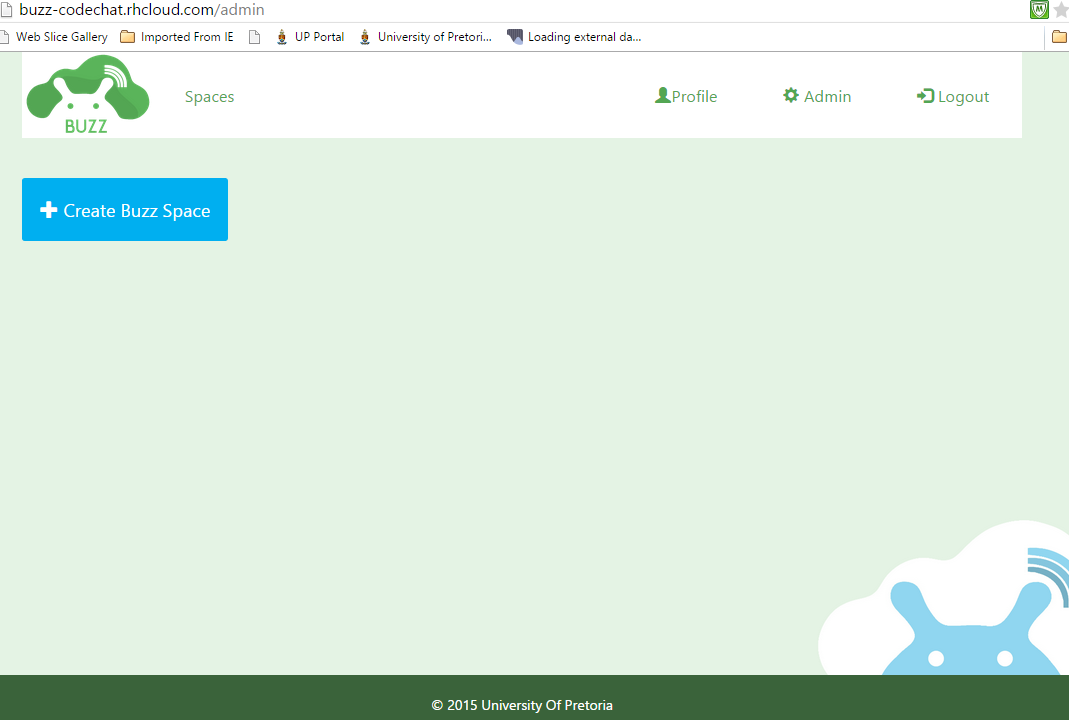
\includegraphics[width=0.5\textwidth,height=4cm]{userswithroles}}
  \caption{User roles in the system }
\end{figure}

\item {spaces}\\
In the buzz space, users are able to view the buzz spaces that are available, no clear distinction of modules registered for and modules they have not yet registered for is presented\\

\begin{figure}[h!]
  \centering
    \reflectbox{%
      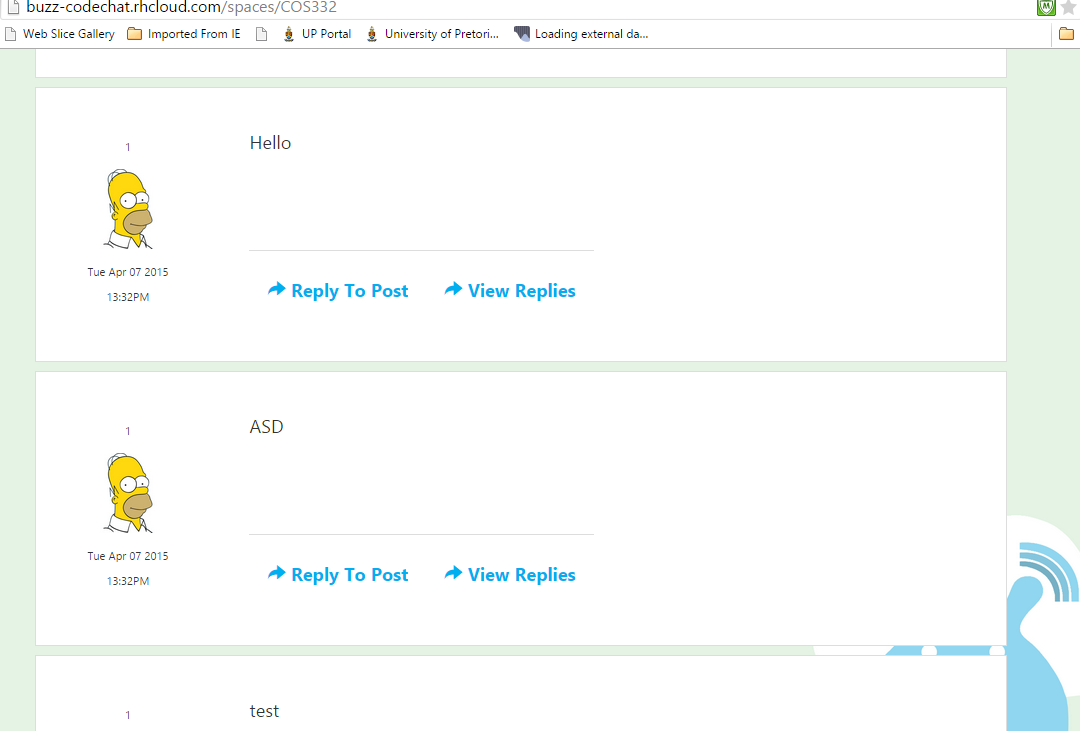
\includegraphics[width=0.5\textwidth,height=4cm]{threads}}
  \caption{threads on the space }
\end{figure}


\item 	UI Considerations around threads\\
Threads are posted as a flat list of posts showing the contents of each posts, no user can post; only view posts hard coded in to the system\\

\item	posts\\
Posts have header, content and footer area, in the buzz space the header contains the user name, the date/time and a profile picture of the user who submitted the post.  The footer contains the submission buttons, no appraisal values, no appraisal types and no posts can be submitted, created or replied to 

\begin{figure}[h!]
  \centering
    \reflectbox{%
      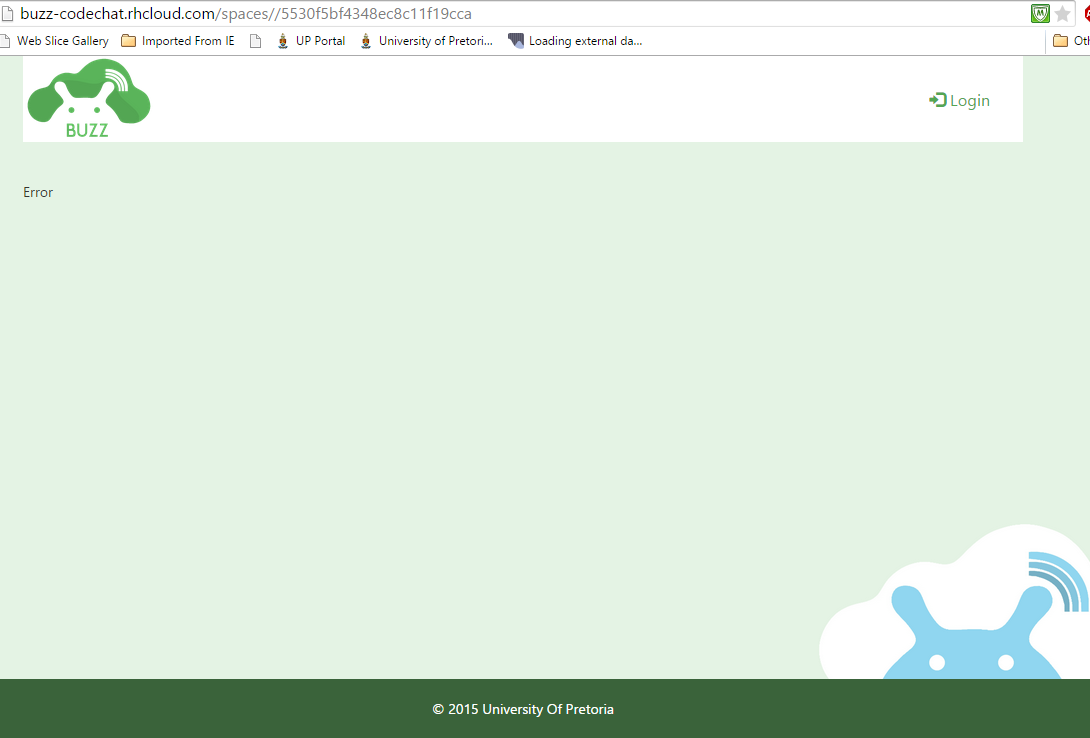
\includegraphics[width=0.5\textwidth,height=4cm]{repytoposterror}}
  \caption{error received when user tries to post }
\end{figure}

 

\item {profile information}\\
A user cab view their own profile picture and are given an option to upload a new one yet that functionality does not work, a user cannot view their user name, role of the user or status and the number of posts/appraisals made/received by the user
\\

 \begin{figure}[h!]
  \centering
    \reflectbox{%
      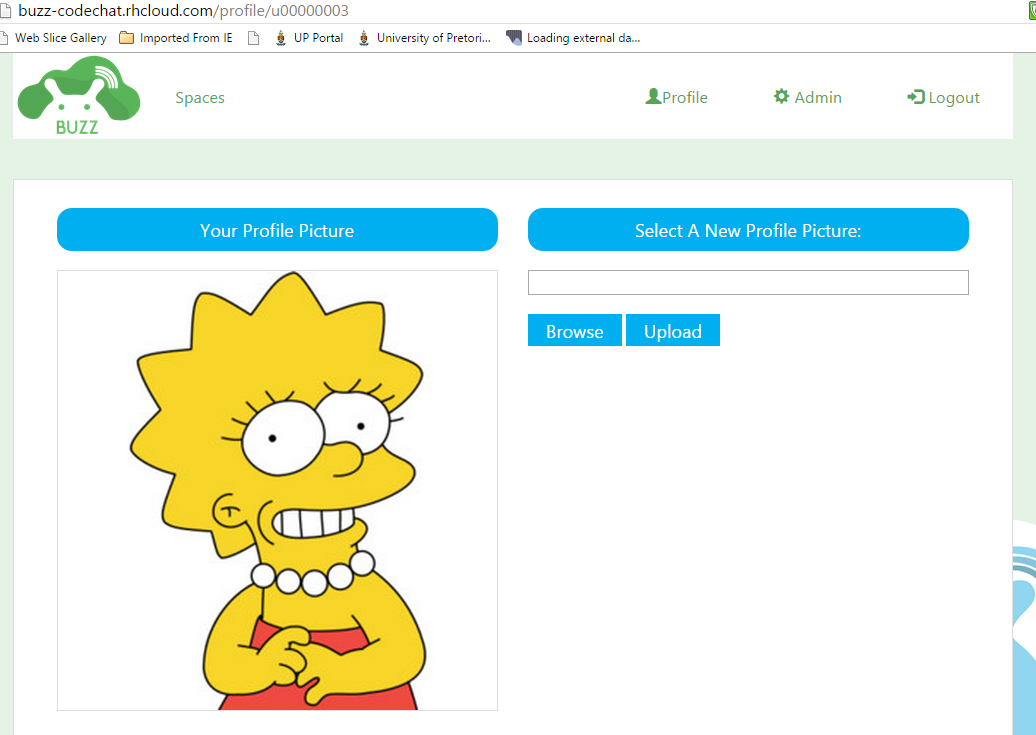
\includegraphics[width=0.5\textwidth,height=4cm]{dummyprofileprovided}}
  \caption{Dummy Profile data }
\end{figure}   


  
\end {itemize}